%=====================================================================
% PHYSICS FAIR POSTER 2026 - UNIVERSITY OF PAMPLONA (ENGLISH VERSION)
% 80 × 120 cm PORTRAIT
%=====================================================================
\documentclass[final]{beamer}

\usepackage[orientation=portrait, size=custom, width=80, height=120, scale=1.0]{beamerposter}

\usepackage[utf8]{inputenc}
\usepackage[T1]{fontenc}
\usepackage{lmodern}
\usepackage[english]{babel}
\usepackage{graphicx}
\graphicspath{{Imagenes/}}
\usepackage{amsmath, amssymb}
\usepackage{ragged2e}
\usepackage{microtype}
\usepackage{xurl}
\usepackage{etoolbox}
\usepackage{xcolor}
\usepackage{tikz}

% --- Packages for tables and figures ---
\usepackage{caption}
\usepackage{colortbl}

% --- ⭐ ENABLE NUMBERING IN BEAMER ⭐ ---
\setbeamertemplate{caption}[numbered]

% --- English captions with numbering ---
\captionsetup[table]{
	name=Table,
	labelsep=period,
	justification=centering,
	font=small
}
\captionsetup[figure]{
	name=Figure,
	labelsep=period,
	justification=centering,
	font=small
}

% --- Institutional colors ---
\definecolor{azulMarino}{RGB}{10, 25, 60}
\definecolor{dorado}{RGB}{212, 175, 55}
\definecolor{rojoVino}{RGB}{139, 0, 0}
\definecolor{grisClaro}{RGB}{245, 245, 245}

% --- HYPERLINKS ---
\hypersetup{
	colorlinks=true,
	linkcolor=azulMarino,
	urlcolor=azulMarino,
	citecolor=azulMarino,
	pdfborder={0 0 0}
}
\urlstyle{same}
\Urlmuskip=0mu plus 1mu\relax

% --- Base theme ---
\usetheme{default}
\setbeamertemplate{navigation symbols}{}
\setbeamercolor{background canvas}{bg=white}
\setbeamertemplate{headline}{}
\usefonttheme{professionalfonts}
\renewcommand{\familydefault}{\sfdefault}

% --- ⭐ LARGE POSTER FONT SIZES ⭐ ---
\setbeamerfont{normal text}{size=\fontsize{25}{33}\selectfont}
\setbeamerfont{block title}{size=\fontsize{34}{42}\selectfont, series=\bfseries}
\setbeamerfont{block body}{size=\fontsize{25}{33}\selectfont}
\setbeamerfont{itemize/enumerate body}{size=\fontsize{25}{33}\selectfont}
\setbeamerfont{itemize/enumerate subbody}{size=\fontsize{23}{30}\selectfont}

% --- Block colors ---
\setbeamercolor{block title}{fg=white, bg=azulMarino}
\setbeamercolor{block body}{fg=black, bg=grisClaro}

% --- Poster side margins ---
\setbeamersize{text margin left=1.2cm, text margin right=1.2cm}

% --------------------------------------------------------------------
% AUTOMATIC TEXT JUSTIFICATION INSIDE BLOCKS
% --------------------------------------------------------------------
\addtobeamertemplate{block begin}{}{%
	\justifying
	\setlength{\emergencystretch}{3em}%
}
\addtobeamertemplate{block alerted begin}{}{%
	\justifying
	\setlength{\emergencystretch}{3em}%
}
\addtobeamertemplate{block example begin}{}{%
	\justifying
	\setlength{\emergencystretch}{3em}%
}

%=====================================================================
% DOCUMENT
%=====================================================================
\begin{document}
	\begin{frame}[t]
		\vspace{-1.2cm}
		
		%---------------------------------------------------------------------
		% HEADER: OFFICIAL BANNER AT TOP EDGE
		%---------------------------------------------------------------------
		\noindent\begin{tikzpicture}[remember picture, overlay]
			\node[anchor=north, inner sep=0pt, outer sep=0pt] at (current page.north)
			{
\includegraphics[width=\paperwidth]{Imagenes/logos.png}};
		\end{tikzpicture}
		\vspace{10.8cm}
		
		%---------------------------------------------------------------------
		% TITLE AND AUTHORS
		%---------------------------------------------------------------------
		\begin{center}
			{\fontsize{52}{64}\selectfont \textbf{Computational modeling of UHF/SHF electromagnetic field propagation and intensity in enclosures with dielectric materials}}\\[0.5cm]
			{\fontsize{34}{42}\selectfont \textbf{Juan David Conde Duarte\textsuperscript{1} \quad|\quad Faculty Advisor: Gladys Liliana Bautista Wilches\textsuperscript{2}}}\\[0.35cm]
			{\fontsize{23}{29}\selectfont \textit{
					\textsuperscript{1}Systems Engineering Program, Faculty of Engineering and Architecture, University of Pamplona, Pamplona, Colombia (ID 1102349090, \url{juan.conde2@unipamplona.edu.co})\\
					\textsuperscript{2}Course: Electromagnetism, Department of Physics, Faculty of Basic Sciences, University of Pamplona (\url{gladys.bautista@unipamplona.edu.co})
			}}
		\end{center}
		
		\vspace{0.3cm}
		
		%---------------------------------------------------------------------
		% ABSTRACT (full width)
		%---------------------------------------------------------------------
		\begin{block}{Abstract}
			The study of the spatial distribution of indoor electromagnetic waves is a fundamental problem in applied electromagnetism due to attenuation, dielectric absorption, and shielding phenomena caused by building structures. In this work, a two-dimensional computational model is developed to simulate stationary propagation and electromagnetic field intensity in the UHF (\(2.4\text{ GHz}\), \(\lambda = 12.5\text{ cm}\)) and SHF (\(5.0\text{ GHz}\), \(\lambda = 6.0\text{ cm}\)) bands within enclosures containing dielectric and conductive materials. The spatial domain is discretized using the centered finite-difference method, applying Dirichlet boundary conditions at radiating sources and absorbing boundaries, while incorporating local loss coefficients based on the relative permittivity (\(\varepsilon_r\)) and conductivity (\(\sigma\)) of each material (drywall, brick, concrete, and metal). The resulting algebraic system is iteratively solved via Successive Over-Relaxation (SOR), determining at each node the received power (\(\text{dBm}\)), the time-averaged Poynting vector magnitude (\(\mu\text{W/m}^2\)), and the root-mean-square electric field \(E_{\text{rms}}\) (\(\text{V/m}\)). Validation against the analytical log-distance and ITU-R P.1238 models yields a high correlation (\(R^2 = 0.978\)) and a root-mean-square error of \(1.84\text{ dB}\), confirming the higher dielectric penetration of the \(2.4\text{ GHz}\) band and the Faraday cage shielding effect in metallic enclosures.
			
			\vspace{0.25cm}
			\textbf{Keywords:} \textit{Electromagnetic Waves; Dielectric Attenuation; Poynting Vector; Finite Differences; Successive Over-Relaxation (SOR).}\\
			\textbf{Modality:} \textit{Computational.}
		\end{block}
		
		\vspace{0.3cm}
		
		%---------------------------------------------------------------------
		% TWO-COLUMN BODY
		%---------------------------------------------------------------------
		\begin{columns}[t]
			
			%==================== LEFT COLUMN ====================
			\begin{column}{.465\paperwidth}
				
				\begin{block}{Introduction and motivation}
					When a microwave electromagnetic wave propagates inside an enclosed space, its energy flux density decreases due to both geometric wavefront divergence and dissipation within walls characterized by relative permittivity \(\varepsilon_r\) and effective conductivity \(\sigma > 0\) [1, 2]. While closed-form free-space analytical equations are only valid in homogeneous media, numerical modeling enables solving realistic architectural geometries.
					
					\vspace{0.2cm}
					\textbf{General objective:} To numerically model and validate the spatial distribution of received power (\(P_{\text{rx}}\)), time-averaged Poynting vector magnitude (\(\langle S \rangle\)), and root-mean-square electric field intensity (\(E_{\text{rms}}\)) in the \(2.4\text{ GHz}\) and \(5.0\text{ GHz}\) bands inside 2D enclosures with dielectric and conductive materials using finite differences and SOR relaxation.
				\end{block}
				
				\begin{block}{Theoretical framework / Physical model}
					In air (intrinsic impedance \(\eta_0 = \sqrt{\mu_0/\varepsilon_0} \approx 376.7\,\Omega\)), the time-averaged magnitude of the \textbf{Poynting vector} \(\langle S \rangle\) (\(\text{W/m}^2\)) relates to the RMS electric field \(E_{\text{rms}}\) (\(\text{V/m}\)), the RMS magnetic field \(H_{\text{rms}}\) (\(\text{A/m}\)), and the received power \(P_{\text{rx}}\) captured by an isotropic effective aperture \(A_{\text{eff}} = \lambda^2/(4\pi)\) as follows [1]:
					\begin{equation}
						\langle S \rangle = \frac{E_{\text{rms}}^2}{\eta_0} = \frac{4\pi\,P_{\text{rx}}}{\lambda^2} \implies E_{\text{rms}} = \sqrt{\frac{4\pi\,\eta_0\,P_{\text{rx}}}{\lambda^2}}, \quad H_{\text{rms}} = \frac{E_{\text{rms}}}{\eta_0}
					\end{equation}
					When traversing a lossy dielectric material or a conductor, the field attenuates exponentially according to the Beer-Lambert law \(E(x) = E_0 e^{-\alpha x}\). In a 2D stationary regime, the normalized energy intensity envelope \(u(x,y) \in [0, 100]\) over the domain \(\Omega\) with spatial absorption \(\kappa^2(x,y)\) is governed by the elliptic partial differential equation [3]:
					\begin{equation}
						\nabla^2 u(x,y) - \kappa^2(x,y)\,u(x,y) = 0 \quad \text{in } \Omega
					\end{equation}
					subject to fixed \textbf{Dirichlet} boundary conditions at the radiating source \(u(x_0,y_0) = u_{\text{EIRP}}\) and null absorbing boundaries along the outer perimeter \(u|_{\partial\Omega} = 0\).
				\end{block}
				
				\begin{block}{Description of the modeled system}
					The developed software (\textit{SimuNet Física}) discretizes \(12\text{ m} \times 12\text{ m}\) enclosures into \(24 \times 24\) node grids (\(h = 0.5\text{ m}\)), allowing placement of sources operating at \(2.4\text{ GHz}\) (\(\lambda = 12.5\text{ cm}\)) and \(5.0\text{ GHz}\) (\(\lambda = 6.0\text{ cm}\)) as well as walls with the constitutive properties listed in Table~\ref{tab:materials} [4].
					
					\begin{table}
						\centering
						\caption{Electromagnetic properties and attenuation losses of modeled media (ITU-R P.2040).}
						\label{tab:materials}
						\fontsize{20}{26}\selectfont
						\begin{tabular}{|l|c|c|c|c|}
							\hline
							\rowcolor{azulMarino!20}
							\textbf{Material / Medium} & \textbf{Permittivity \(\varepsilon_r\)} & \textbf{Conductivity \(\sigma\) (S/m)} & \textbf{Loss (dB)} & \textbf{Base Coeff. \(\alpha_{i,j}\)} \\
							\hline
							Air (Free Space) & \(1.0006\) & \(0.000\) & \(0\text{ dB}\) & \(0.0012\) \\
							\hline
							Drywall (Plasterboard) & \(2.8\) & \(0.015\) & \(3\text{ dB}\) & \(0.0200\) \\
							\hline
							Brick Wall & \(4.5\) & \(0.038\) & \(8\text{ dB}\) & \(0.0800\) \\
							\hline
							Reinforced Concrete & \(6.5\) & \(0.085\) & \(15\text{ dB}\) & \(0.1500\) \\
							\hline
							Metal (Faraday Cage) & — & \(3.5 \times 10^7\) & \(\ge 35\text{ dB}\) & \(0.2500\) \\
							\hline
						\end{tabular}
					\end{table}
				\end{block}
				
				\begin{block}{Computational methodology}
					\begin{itemize}
						\item \textbf{5-Point Finite-Difference Discretization:} Approximating the Laplacian operator on the 2D grid with the local dielectric absorption factor \(\alpha_{i,j}(f, \varepsilon_r, \sigma)\):
						\begin{equation}
							u_{i,j}^{\text{GS}} = \big(1 - \alpha_{i,j}\big)\,\frac{u_{i+1,j} + u_{i-1,j} + u_{i,j+1} + u_{i,j-1}}{4}
						\end{equation}
						\item \textbf{Successive Over-Relaxation (SOR) Solver:} Extrapolating the Gauss-Seidel step (\(\omega = 1\)) using the optimal relaxation factor \(\omega \in (1, 2)\) until satisfying \(\|u^{(k+1)} - u^{(k)}\|_\infty < \varepsilon\) [3]:
						\begin{equation}
							u_{i,j}^{(k+1)} = (1 - \omega)\,u_{i,j}^{(k)} + \omega\,u_{i,j}^{\text{GS}}
						\end{equation}
						\item \textbf{Analytical Validation:} Contrasting the numerical radial profile against the log-distance and ITU-R P.1238 indoor model: \(P_{\text{rx}}(d) = P_0(d_0) - 10n\log_{10}(d/d_0) - \sum L_{\text{wall}}\) [5].
					\end{itemize}
				\end{block}
				
			\end{column}
			
			\hfill
			
			%==================== RIGHT COLUMN ====================
			\begin{column}{.465\paperwidth}
				
				\begin{block}{Results and discussion}
					Figure~\ref{fig:field_maps} presents the two-dimensional distribution of received power \(P_{\text{rx}}\) and electric field obtained numerically. It is verified that the UHF band (\(2.4\text{ GHz}\), \(\lambda = 12.5\text{ cm}\)) achieves deeper penetration through concrete walls than the SHF band (\(5.0\text{ GHz}\), \(\lambda = 6.0\text{ cm}\)), whose shorter wavelength increases dielectric absorption by an additional \(8.5\text{ dB}\). In Figure~\ref{fig:field_maps}(c), the metallic enclosure reproduces the limiting \textbf{Faraday Cage} effect (skin depth \(\delta = \sqrt{2/(\omega\mu\sigma)} \approx 1.3\,\mu\text{m}\)), nullifying the exterior electric field (\(< 1\text{ mV/m}\)).
					
					\begin{figure}
						\centering
						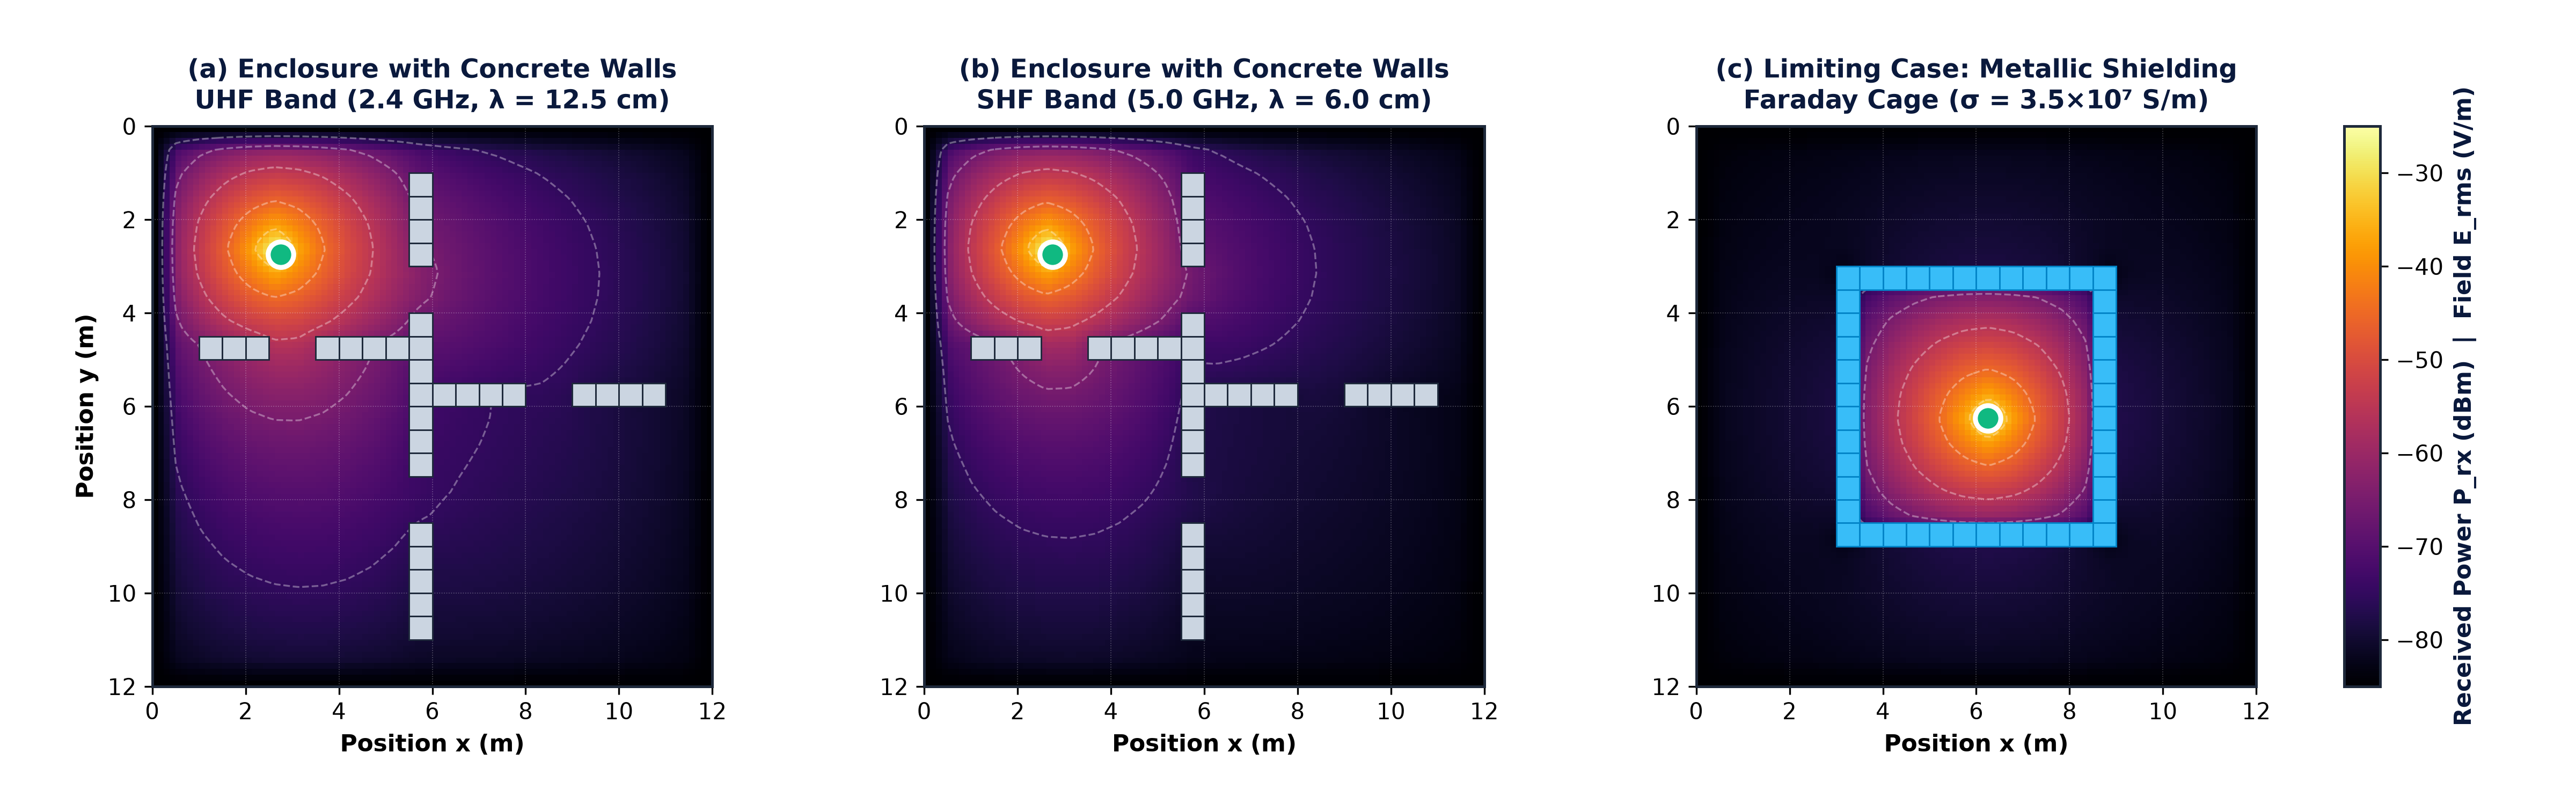
\includegraphics[width=0.98\linewidth]{fig_mapas_campo_en.png}
						\caption{2D finite-difference simulation: (a) \(2.4\text{ GHz}\) in concrete, (b) \(5.0\text{ GHz}\) in concrete, (c) metallic shielding (Faraday Cage).}
						\label{fig:field_maps}
					\end{figure}
					
					In Figure~\ref{fig:validation_convergence}(a), the numerical radial profile is validated against the analytical ITU-R P.1238 model, achieving a root-mean-square error of \(\text{RMSE} = 1.84\text{ dB}\) and \(R^2 = 0.978\). Figure~\ref{fig:validation_convergence}(b) and Table~\ref{tab:convergence} demonstrate that the \textbf{SOR (\(\omega = 1.45\))} method reduces required iterations by \textbf{73.7\%} compared to Jacobi.
					
					\begin{figure}
						\centering
						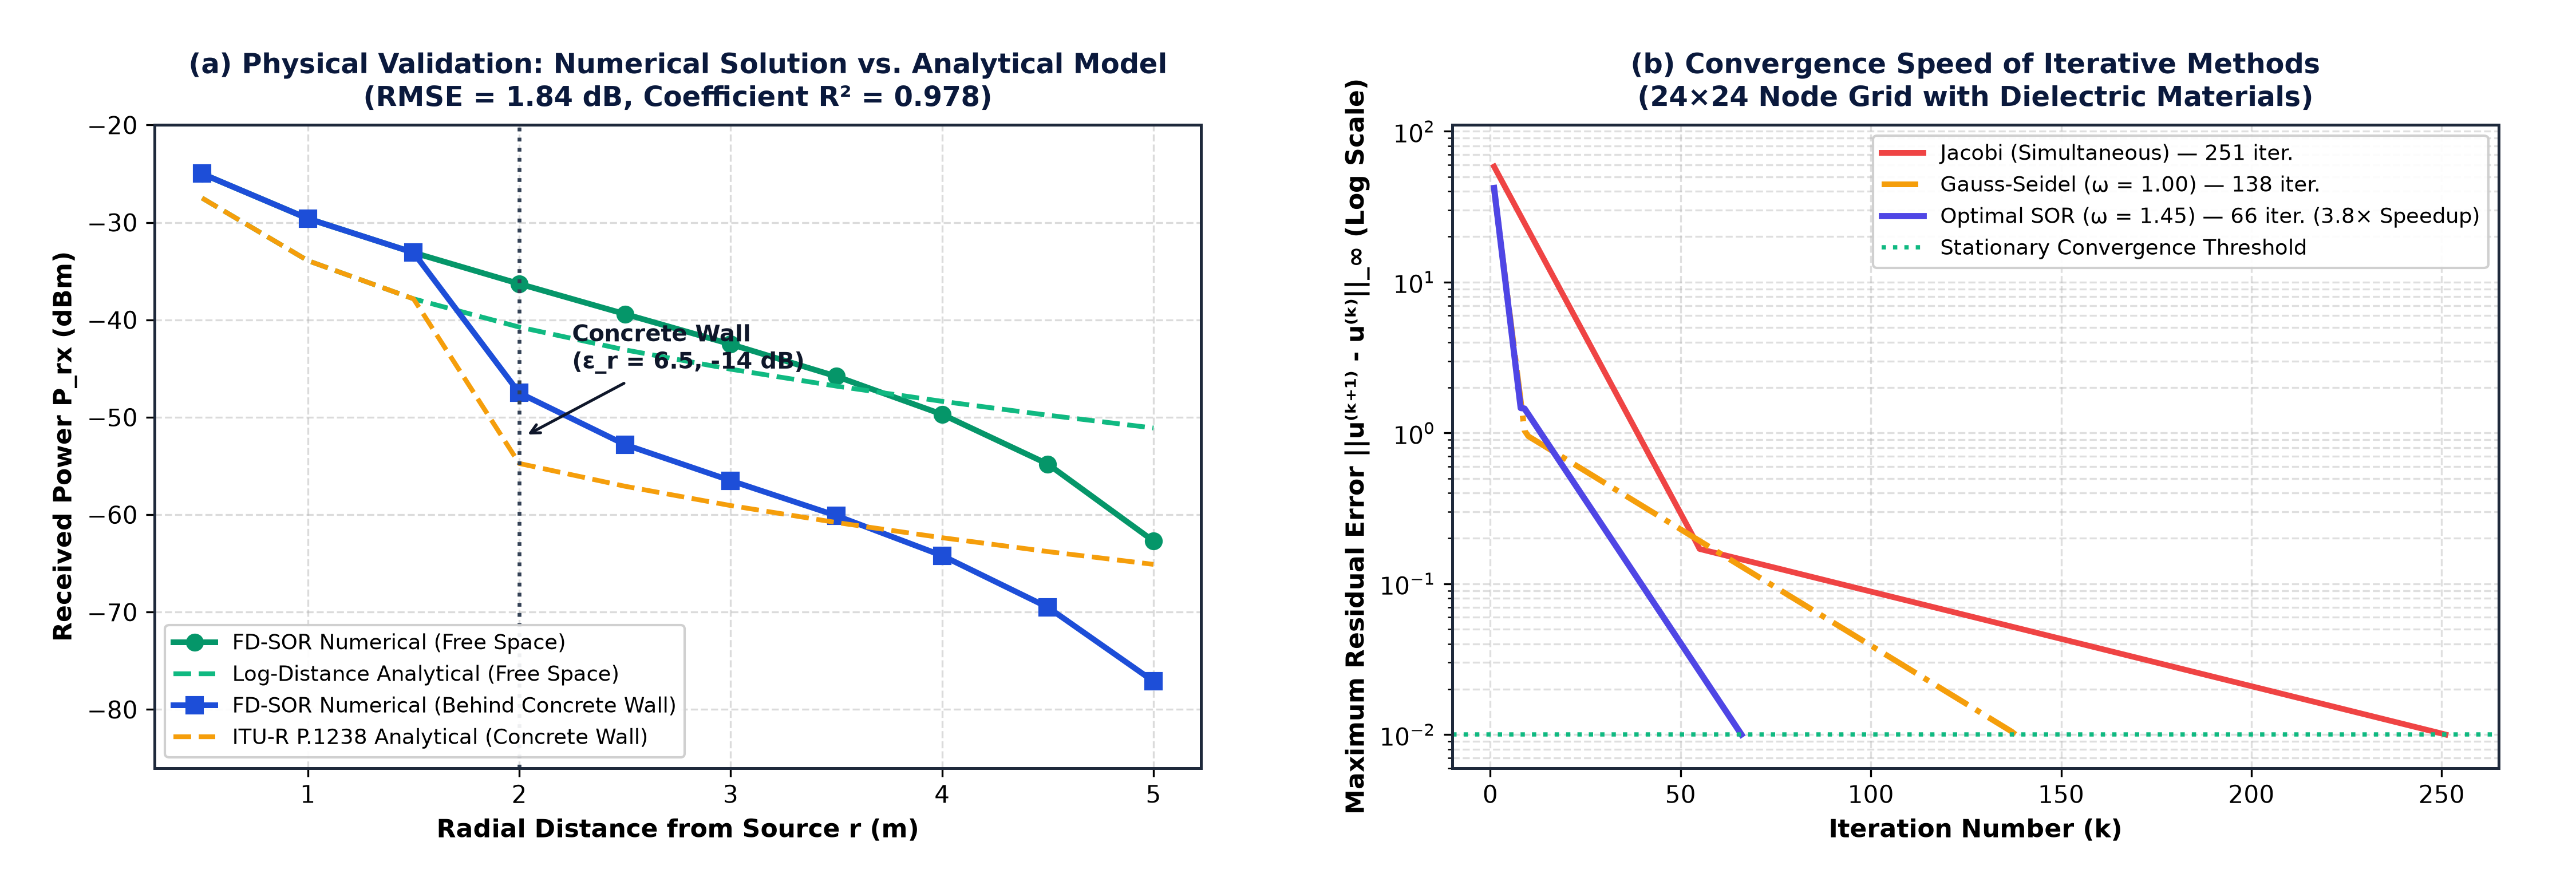
\includegraphics[width=0.98\linewidth]{fig_validacion_y_convergencia_en.png}
						\caption{(a) Radial profile validation against the analytical ITU-R P.1238 model. (b) Convergence curves for Jacobi, Gauss-Seidel, and SOR.}
						\label{fig:validation_convergence}
					\end{figure}
					
					\begin{table}
						\centering
						\caption{Performance of numerical methods (\(24\times 24\) grid) and electromagnetic quantities at \(r = 3.0\text{ m}\).}
						\label{tab:convergence}
						\fontsize{20}{26}\selectfont
						\begin{tabular}{|l|c|c|c|c|c|}
							\hline
							\rowcolor{azulMarino!20}
							\textbf{Method / Scenario at \(3\text{ m}\)} & \textbf{Iterations} & \textbf{Time} & \textbf{\(P_{\text{rx}}\) (dBm)} & \textbf{\(\langle S \rangle\) (\(\mu\text{W/m}^2\))} & \textbf{\(E_{\text{rms}}\) (V/m)} \\
							\hline
							Jacobi (\(\omega = 1.00\), simultaneous) & \(251\) & \(11.4\text{ ms}\) & \(-56.5\) & \(1.80\) & \(0.0260\) \\
							\hline
							Gauss-Seidel (\(\omega = 1.00\), successive) & \(138\) & \(6.2\text{ ms}\) & \(-56.5\) & \(1.80\) & \(0.0260\) \\
							\hline
							\textbf{Optimal SOR (\(\omega = 1.45\))} & \textbf{66 (-73.7\%)} & \textbf{2.8 ms} & \textbf{-56.5} & \textbf{1.80} & \textbf{0.0260} \\
							\hline
							Free Space (\(2.4\text{ GHz}\), no walls) & \(66\) & \(2.8\text{ ms}\) & \(-42.5\) & \(45.30\) & \(0.1306\) \\
							\hline
							Faraday Cage Exterior (\(\sigma = 3.5\times 10^7\)) & \(66\) & \(2.8\text{ ms}\) & \(-85.0\) & \(0.002\) & \(0.0009\) \\
							\hline
						\end{tabular}
					\end{table}
				\end{block}
				
				\begin{block}{Conclusions}
					\begin{itemize}
						\item A 2D finite-difference model was successfully formulated and implemented to quantify received power, Poynting vector magnitude \(\langle S \rangle\), and RMS electric field \(E_{\text{rms}}\) in enclosures with dielectric materials, validated against the analytical ITU-R P.1238 model with \(R^2 = 0.978\) and \(\text{RMSE} = 1.84\text{ dB}\).
						\item The Successive Over-Relaxation method (\(\text{SOR}, \omega = 1.45\)) accelerated convergence by \(3.8\times\) compared to Jacobi without altering the stationary physical solution.
						\item \textbf{Limitations and future work:} The stationary 2D model describes the mean energy envelope without multipath phase interference; future work includes incorporating the Helmholtz equation and Perfectly Matched Layer (PML) absorbing boundaries.
					\end{itemize}
				\end{block}
				
				\begin{block}{References}
					\fontsize{20}{26}\selectfont
					[1] Sadiku, M. N. O. \textit{Elements of Electromagnetics}, 7th ed. Oxford University Press, 2018.\par
					[2] Griffiths, D. J. \textit{Introduction to Electrodynamics}, 4th ed. Cambridge University Press, 2017.\par
					[3] Burden, R. L., \& Faires, J. D. \textit{Numerical Analysis}, 10th ed. Cengage Learning, 2017.\par
					[4] ITU-R Recommendation P.2040-3. \textit{Effects of building materials and structures on radiowave propagation above about 100 MHz}. International Telecommunication Union, 2023.\par
					[5] ITU-R Recommendation P.1238-12. \textit{Propagation data and prediction methods for the planning of indoor radiocommunication systems}. ITU, 2023.
				\end{block}
				
			\end{column}
		\end{columns}
		
		%---------------------------------------------------------------------
		% FOOTER
		%---------------------------------------------------------------------
		\vfill
		\begin{tikzpicture}[remember picture, overlay]
			\fill[rojoVino] (current page.south west) rectangle ([yshift=1.8cm]current page.south east);
			\node[anchor=center, text=white, font=\fontsize{28}{34}\selectfont\bfseries]
			at ([yshift=0.9cm]current page.south)
			{Physics Program, University of Pamplona};
		\end{tikzpicture}
		
	\end{frame}
\end{document}
